\section{Harris}\label{sec:harris}
Harris hjørnedetektor blev introduceret af Chris Harris og Mike Stephens i 1988 \cite{harris}. Detektoren kan ses som en videreudvikling af Moravec, da den adresserer Moravecs begrænsninger:
\begin{enumerate}
\item{ \textit{Anisotropisk respons:} Harris og Stephens udvider Moravecs udregning af auto-korrelation til at måle intensitetsvariationer i alle retninger. Auto-korrelationen imellem skiftende vinduer kan approksimeres ved at udvide funktionen, ved en Taylor udvidelse af anden orden, og beskrives derved udefra dens afledte:
\begin{subequations}
\begin{align}
E(u,v) = & \sum w(x,y)[I(x + u, y + v) - I(x,y)]^2 \\
\approx & \sum w(x,y)[I(x,y) + uI_x  + vI_y - I(x,y)]^2 \\
= & \sum w(x,y)[u^2I_x^2 + 2uvI_xI_y + v^2I_y^2]  \label{last}
\end{align}
\end{subequations}
Ligning \eqref{last} kan omskrives til matrixformen
\begin{equation}
E(u,v) \approx
\begin{bmatrix}
        u & v
     \end{bmatrix}
M
\begin{bmatrix}
        u \\
        v
     \end{bmatrix}
\end{equation} 
Hvor $M$ er auto-korrelations matricen (også kaldt struktur-tensoren), med $w(x,y)$ ganget på:
\begin{equation}
M = w(x,y) 
\begin{bmatrix}
	I_x^2 & I_xI_y \\
	I_xI_y & I_y^2
\end{bmatrix}
\label{structens}
\end{equation}
Billedets afledte i $x$ og $y$ aksen findes ved at udføre en diskret differentiering af billedet, hvilket kan opnås
 ved at folde billedet, med henholdsvis $[-1 \hspace{0.1cm} 0 \hspace{0.1cm} 1]$ og $[-1 \hspace{0.1cm} 0 \hspace{0.1cm} 1]^T$. }
\item{\textit{Støj sensitiv:} Harris detektoren anvender et Gaussisk vindue $w(x,y)$ omkring det undersøgte pixelområde. Det Gaussiske vindue anvendes til at fjerne støj fra billedet.}
\item{\textit{Højt kant respons} Struktur-tensoren 'M' opskrevet i \eqref{structens} indeholder de kvadrerede differentierede retninger i et givet punkt og derved en beskrivelse af billedets geometriske struktur, i et punkt $(x,y)$. Egenværdierne for denne matrix, vil være proportionale med de forskellige steder vinduet kan placeres:
\begin{itemize}
\item{ \textit{Homogen flade.} Billedintensiteten er konstant. Begge egenværdier vil være små.}
\item{\textit{Kant.} For punkter placeret på en kant, vil der være en stor krumning på tværs af kanten, men ingen når kanten følges. Derfor vil én egenværdi være stor, mens den anden vil være lille}
\item{\textit{Hjørne.} Et punkt placeret på et hjørne, vil have en stor krumning, i hver retning og derved bestå af to store egenværdier.}
\end{itemize}
Det ønskes derfor, for at identificere hjørner, at begge egenværdier for M er store. Egenværdierne kan defineres ud fra determinanten og sporet af M:
\begin{subequations}
\begin{align}
\textbf{det}M & = \lambda_1 \lambda_2 \\
\textbf{trace}M & = \lambda_1+\lambda_2
\end{align}
\end{subequations}
Harris og Stephens foreslår et mål for hjørnestyrken, baseret på forholdet imellem de to egenværdier. En høj værdi for hjørnestyrken angiver to store egenværdier. Forholdet mellem egenværdierne kan defineres således:
\begin{equation}
R = \textbf{det}M-k(\textbf{trace}M)^2
\label{rvalharris}
\end{equation}
hvor \textit{k} er en empirisk defineret konstant udledt af Harris og Stephens som ligger i intervallet $[0.04,0.06]$. I figur \ref{fig:egen} ses sammenhængen mellem værdien $R$, egenværdierne og hvordan de korrespondere med hjørner, kanter og homogene områder, igen kan det ses at for et hjørne ønskes to store egenværdier.
\begin{figure}[H]
    \centering
    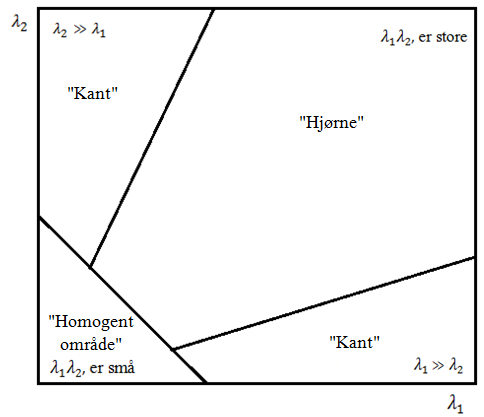
\includegraphics[width=0.45\textwidth]{fig/26.png}
     \vspace{-1em}
    \begin{center}    
       \caption{{\footnotesize \textit{Sammenhængen imellem struktur tensorens egenværdier og forskellige strukturer.}}}
    \label{fig:egen}
     \end{center}
     \vspace{-2.5em}
  \end{figure} \noindent
Ved værdien for R, kan det defineres om et punkt er lokaliseret på et hjørne. De interessante hjørne, er hvor der opstår en stor hjørnestyrke, hvilket kan findes ved at sætte en grænseværdi $t$, der definere om et hjørne er lokaliseret(sandt/falsk).
\begin{equation}
\begin{split}
\texttt{hjørne} = 
\begin{cases}
\texttt{sandt}& \text{hvis } R\geq t, \\
\texttt{falsk }& \text{hvis } R < t.
\end{cases}
\end{split}
\label{cornerhar}
\end{equation}
}
\end{enumerate}
\subsubsection*{Algoritme: Harris Detektor}
\begin{tabbing}
Input\quad \= : \= Billede $I$\\
Output \text{ } \> : \> Interessepunkter $p \in (x,y)$
\end{tabbing}
\begin{enumerate}
\item{For hver pixel i billedet $(x,y)$, udregnes struktur tensoren, beskrevet i ligning \eqref{structens}}
\item{For hvert pixel i billedet udregnes hjørnestyrken ved ligning \eqref{rvalharris}.  Hvis den udregnede hjørnestyrke opfylder ligning \ref{cornerhar}, for en given grænseværdi, udvælges punktet som værende et hjørne.}
\end{enumerate}
\subsection*{Konklusion}
Metoden anvendes som en repeterbar detektor og bruges i høj grad i dag. Detektoren er rotationsinvariant pga. dens brug af egenværdier, men er ifølge \cite{eval} stadig delvis anisotropisk, hvilket skyldes differentierings filtrene, der kun udledes i $x$ og $y$ retningen. Mikolajczyk og Schmid \cite{eval1} konkludere at detektoren er særlig følsom over for rotation omkring 45 grader. De konkludere også at detektorens repeterbarhed falder drastisk ved skalaændringer.